%***************************************************************************
% Chapter 2 of pluginarch.tex
% Authors: Remy Muller & Vincent Goudard
%***************************************************************************

\chapter{What is an audio plugin?}


%---------------------------------------------------------------------------
\subsubsection{What is its purpose?}
\noindent A plugin is intended to extend an audio creation environment by the use of dedicated third party libraries. Thus any user should be able to find plugins that fits perfectly their needs to customize this environment. Typically plugins can be considered as \textit{virtual devices} based on the analogy with hardware devices such as reverbs, compressors, delays, synthetizers, samplers or beatboxes that can be connected together in a modular way. This allows host manufacturers to focus on the conviviality and efficiency of their products while specialized manufacturers rather focus on the \textit{Digital Signal Processing} part.

\subsubsection{Approaches}
We can distinguish 3 approaches to do plugins
\begin{itemize}
\item Plugins integrated into a multimedia API like Apple's Audiounits and Microsoft's DirectX. 
\item Plugins related to a reference host like VST, RTAS, MAS\footnote{respectively cubase, protools and digital performer}. Some of them can be found on different plateforms like VST or RTAS.
\item Modules attached to modular softwares like the "Max family"\footnote{Cycling 74's Max/Msp, Ircam's jMax an CRCA's Pure Data.}, Buzz or EyesWeb.
\end{itemize}
We should also consider LADSPA on GNU-linux which is the de-facto standard for that plateform but that can not be attached to any  of the above categories.


%---------------------------------------------------------------------------
\section{General model}
\noindent A plugin treats an \textbf{audio signal} then it needs to be \textbf{controlled} and in order to work in a host environment, host and plugin have to know their repective {setup \& properties}.\\
The audio stream is usually treated by blocks (buffers) inside whom samples are synchronous to the samplerate. In general, control parameters have a lower refresh rate and can be either treated between audio blocks -- on-demand -- if the value has changed, or queued with time-stamps relative to a position in a block for audio-rate resolution. Properties are mostly static flags but some can be dynamic though.\\

\begin{figure}[htb]
\begin{center}
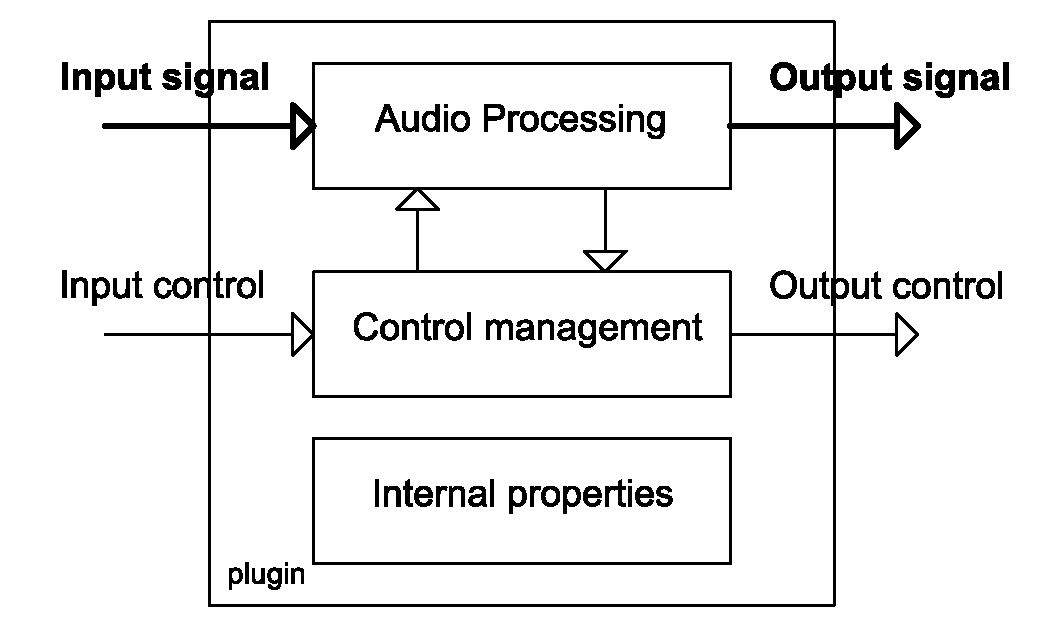
\includegraphics[height=2.5in,width=4.16in]{pluginmodel}
\caption{A common model behind musical plugin architetures}
\end{center}
\end{figure}

\subsubsection{Setup \& properties}
\noindent Plugins have to know about the host's capabilities like sending/receiving events, providing multichannels busses\ldots  In addition there are lot of situations where we would appreciate that plugins can know more about the \textit{musical context} (i.e. tempo, score-position, metric\ldots) than just audio and control data.\\
\noindent The plugin has to give information about its ins/outs, their specificities such as side-chain, mono, stereo or surround and many things such as its latency\footnote{An algorithm like a Fourrier Transform may introduce a pure delay in the signal chain because it needs a minimum number of sample to start. In a sequencer (not in real-time!) this pure delay can be compensed by the host by sending data to the plugin in advance.} or its tail-time\footnote{Basically all the algorithms based on convolution may introduce a tail i.e. output samples even when there is no more input data (e.g. a delay, a reverb a FIR filter\ldots)}. There is also some hosts that allow plugins to give them commands such as \textit{play, stop or set tempo} but it is not really wide-spread. 


%---------------------------------------------------------------------------
\section{Inputs -- Outputs}
 
\noindent To understand what is relevant to determine the number and the kind of IOs, we may analyse what plugins algorithms does around 3 different of kind functionnalities -- analysis (\textbf{A}), transformation (\textbf{T}) and synthesis (\textbf{S}) -- that can be either alone or mixed together in the same entity.\\

\begin{figure}[htb]
\begin{center}
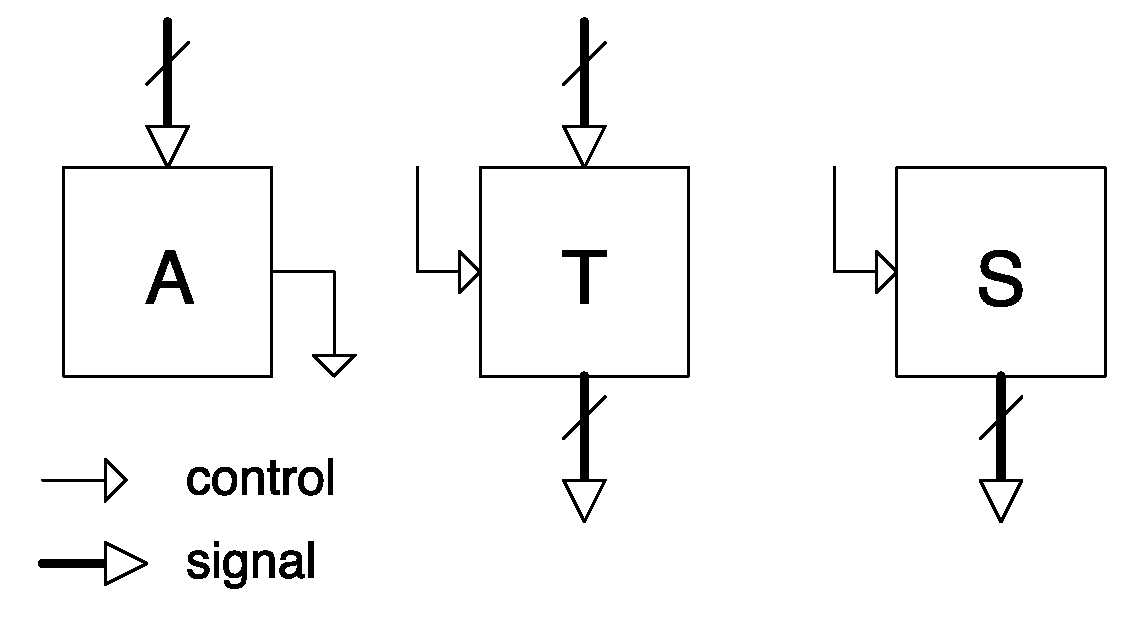
\includegraphics[height=1.2in,width=2.2in]{functions}
\caption{functions}
\end{center}
\end{figure}  

\noindent Moreover, plugin setups highly depend on what the host allows and how the plugin will be attached to its environment. While most hosts only support mono and stereo (even if surround begins to be popular with  the recent success of the DVD and the famous 5.1 surround format\footnote{left, center, right, rear left, rear right plus subwoofer}), we can also distinguish between effects that will be treated as \textbf{inserts} (integrated in a chain on a single bus), \textbf{sends} (they can be shared by many voices in a mixing-console and the output is summed on the master bus), \textbf{instruments} (no audio input) or simply integrated into a modular host.

\subsubsection{Audio}
\noindent The number of \textbf{audio inputs and outputs} vary from one plugin to another, they can be grouped into busses that can be mono, stereo, surround\ldots but they mostly depends on the host capabilities. Moreover, in some standards -- the number is still growing --, it is possible to define side-chain\footnote{a side-chain channel can be analyzed or used directly to modify the main audio stream processing.} (see figure \ref{sidechain}). 

\begin{figure}[htb]
\begin{center}
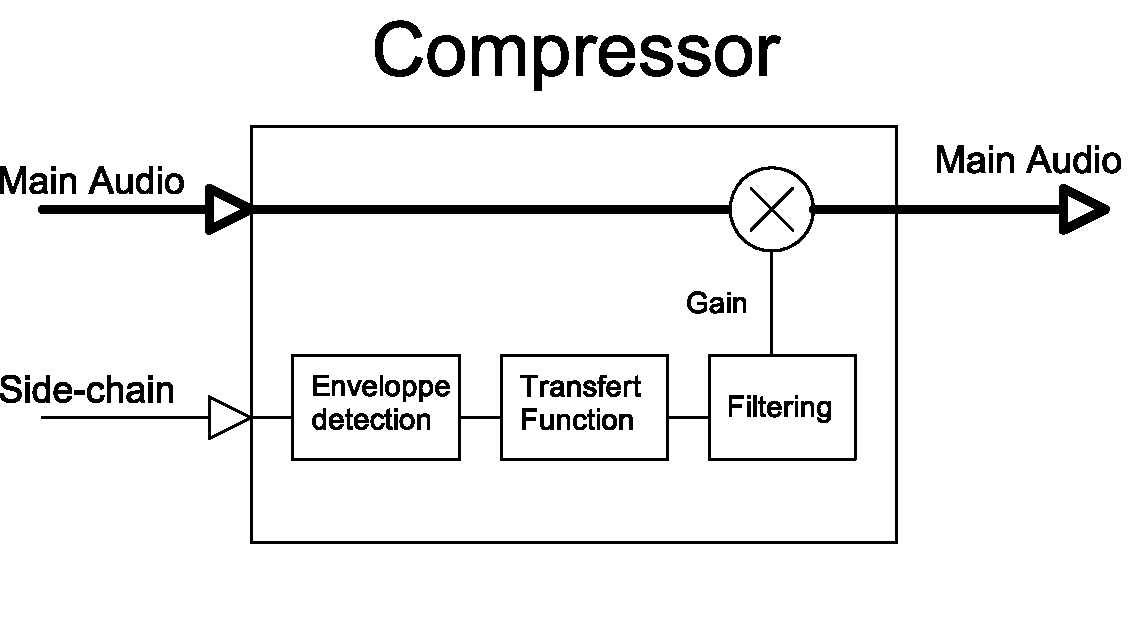
\includegraphics[height=2in,width=3.5in]{sidechain}
\caption{A side-chain example: a compressor}
\label{sidechain}
\end{center}
\end{figure}  

\subsubsection{Control}
\noindent Though it is possible to build a plugin that has no way to be controlled, like a phase inverter, it is of limited interest in a musical context where tweaking the parameters or sending notes is part of the creation. You may want to both change the plugin's parameters and record their variation for later playback. Hence most plugins should provide control input and output at the same time. Most of the time hosts and plugins notify each other of parameters' evolution in a simple way but one can also find callback and polling mechanisms. In addition sending \textbf{control data} between plugins can sometimes be performed either directly via parameters (LADSPA) or by an event-oriented protocol like MIDI (VST).\\

%---------------------------------------------------------------------------
\section{The ``process"}
\noindent All plugins have this function in common often called ``process''. This is where the most important thing happens: \textit{audio processing}.
All the current standards treat audio as input and output buffers (of given length), that can be given as floating-point sample arrays, or by more sophisticated structures with additionnal information. Processing can be in-place, in which case in and output buffers are the same (i.e. they share the same memory location, processing is thus destructive.), or buffer-to-buffer, where they are different in this case it is possible to have either accumation (send effects) or replacing (inserts). Parameters are usualy known before the process starts, but you may have to update them by hand. For simple audio processing like biquadratic filtering, it should be enough to use directly the buffer provided, but when doing FFT processing for example you may want to re-buffer audio samples to fit your internal buffer size in which case you may introduce additionnal latency in the signal chain.

%...........................................................................
\section{The user interface}
\noindent The GUI should be considered at least as important as the audio processing algorithm because it is the filter thru wich your plugin will be perceived. It is a key-point for the conviviality and usability of a plugin, everything should be fast and easily tuneable in a precise way with a convenient visual feedback. In particular, parameters' mapping can really make the difference in the way people feel about how your plugin sounds.\\
% citer les �tudes psycho-acoutiques sur l'influence du mapping.
The GUI can be either generated automatically by the host with the help of the information or hints that the plugin can provide about itself (its  parameters type, their range and units\ldots, and the type of control that should be used -- slider, combo-box, switch, knob, 2D controler, \ldots --) or provided by the plugin manufacturer to reach a higher level of customization.\\
However we will skip the GUI topic in this document. We consider control parameters as the plugin interface without taking account the way these parameters are changed by the user.

%...........................................................................
\section{Plugin developpement}
\noindent The API defines the layer through which plugins and hosts can see each other and also the tools that can be used to ease the developpement step.\\
The Host needs different information than the user about plugins such as their ID, their capabilities, their setup, the number of parameters or their names. The host needs to receive computer-readable data in the way it is programmed to. In addition most of the SDKs\footnote{Software Developpement Kits.} provide a set of tools, functions, utilities. In the same effort, they often allow the use of OOP\footnote{Object Oriented Programming.} languages such as C++, ObjectiveC or Pascal to ease the modelisation step and the tasks distribution inside a same plugin.
%----------------------------------EOF-------------------------------------%